\vspace{1cm}
 Our system is based on a client/server architecture with three layers. Presentation, application and data access are physically separated. We choose this kind of architecture in order to have a modular system, also we use fat client to reduce the server load and smartphones nowadays are very powerful so, the costs of server will be less. Moreover we separated physically the database from the application server, to increase scalability and security, and it’s also possible to use a distributed database. This choices promote a major decoupling of the system, increasing the reusability, scalability and flexibility. Furthermore, components in the application server have been thought to be cohesive and with low coupling among modules to make the system more comprehensible and modifiable. \\ \\
 The communication between the Mobile application and the Server will be done via HTTP requests following REST principles. The communication between modules inside the application server and DB manager is RPC. When we use RPC, the programmer can use procedure call semantics and writing distributed applications is simplified because RPC hides all of the network code into stub functions.\\ \\
 In addition, we use some caches in the client side so we avoid some interactions between the client and server so we could reduce server loads. For example, in a short period of time users location do not change so, we could cache shops near the user for short amount of time and do not send requests to server.\\ \\
 We use JSON format for the communication data because, JSON uses less data overall, so you reduce the cost and increase the parsing speed. Readable: The JSON structure is straightforward and readable. You have an easier time mapping to domain objects, no matter what programming language you're working with.\\ \\
 The model we choose for this project is Model View Controller (MVC). This model improves the reusability and maintainability of code. One of the most important feature of this design pattern is separation of concerns. 
 \begin{itemize}
     \item \textbf{View} is that part of the application that represents the presentation of data. Views are created by the data collected from the model data. A view requests the model to give information so that it resents the output presentation to the user.\\
     
     \item \textbf{Controller} is that part of the application that handles the user interaction.
     
     \item \textbf{Model} component stores data and its related logic. It represents data that is being transferred between controller components or any other related business logic.
     
 \end{itemize}
 \begin{figure}[H]
  \centering
  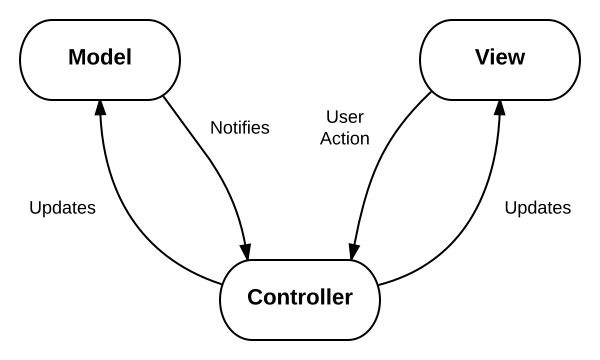
\includegraphics[width=0.8\textwidth,keepaspectratio]{images/all/MVC.png}
  \caption{Model View Controller}
\end{figure}